\section{Duality: DNNs are both layers as well as paths}
In this paper, we look at DNNs with ReLU. A special property of ReLU is that it is also a gate which either blocks (i.e., multiplies by $0$) or allows (i.e., multiplies by $1$) its pre-activation input. A consequence of the gating property is \emph{duality}: DNNs are layers as well as paths. A path starts at an input node, passes through gates and weights and ends at the output node and the output can be expressed as a summation of individual path contributions. \cite{npk} used duality to separate the gates as masks from the weights and argued (via experiments and theory) that \emph{gates of a DNN alone is enough to obtain power insights}. The key experimental and theoretical results are summarised in the next two points.

1. \textbf{Experimental:} Using a deep gate network to decouple the gates as masks from the weights, it was shown that  (i) gates are learnt during training, (ii) learnt gates generalise better, (iii) most information is in the gates, i.e., with learnt gates as masks the weights can be reset and retrained without significant loss in test accuracy (iv) learning in gates is the reason why finite width DNNs perform better than infinite width NTK.


2.  \textbf{Theoretical:}  When the gates are decoupled from weights, the NTK is a summation of two kernels, i.e., NTK = $\text{NTK}^{\text{fixed-gate}}+ \text{NTK}^\text{gate-learning}$, where $\text{NTK}^{\text{fixed-gate}}$ is the kernel that corresponds to learning the wights keeping the gates fixed and $\text{NTK}^\text{gate-learning}$ is the kernel corresponds to learning of the gates themselves. Main theorem shows that the $\text{NTK}^{\text{fixed-gate}}$ simplifies into a \emph{neural path kernel} (NPK), which measures the similarity of a given pair of input examples in terms of the size of sub-network that is active\footnote{Active sub-network comprises of the gates which are \emph{on} (i.e., $1$) and the weights connecting such gates.} simultaneously for both the input examples.  


Since we will be using the dual view, we now provide a brief summary of the same.

\begin{comment}
Rewriting everything in terms of gates.
Simple Theory: Kernel depends on only gates. NTK = NPK

Simple Experiments: Instead of designing another kernel method based on NPK we have 2 choices i) design another kernel ii) use the observation to more simple experiments. that NPK Keep experimenting with various gating patterns.

\end{comment}
\subsection{Neural Path Features and Value: Fully Connected}
\FloatBarrier
\begin{figure}[h]
\centering
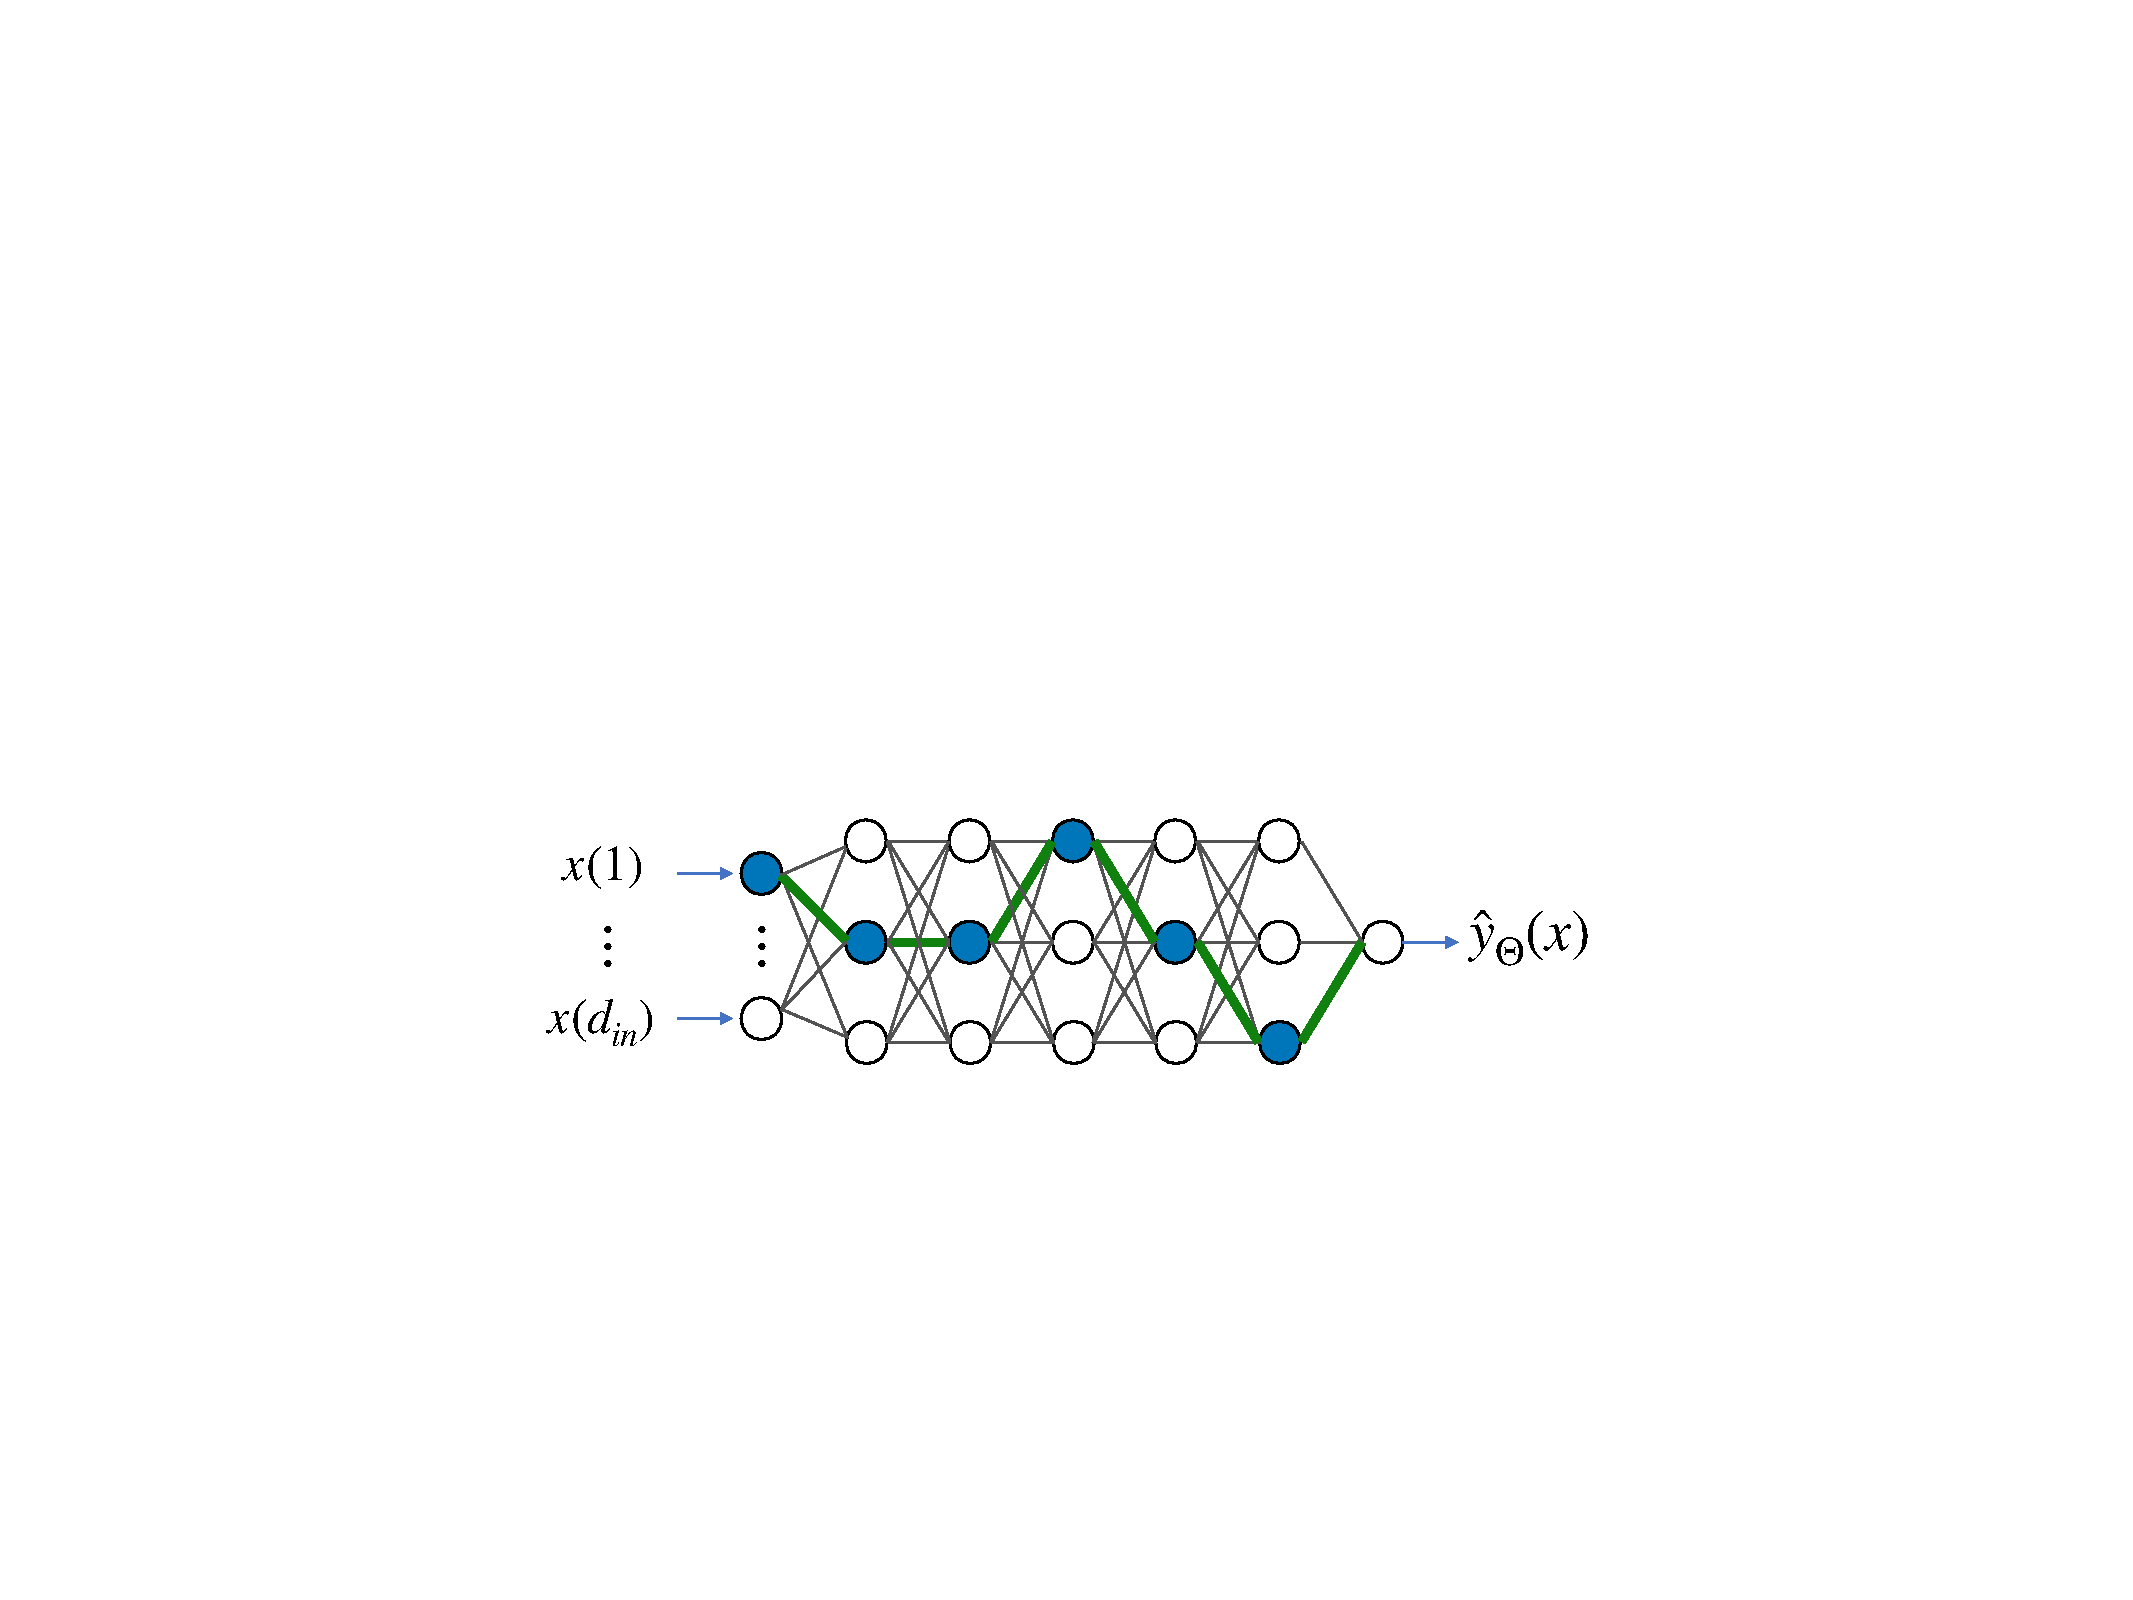
\includegraphics[scale=0.32]{figs/paths.pdf}
\end{figure}
A path starts from an input node, passes through exactly one weight and one hidden node in each layer and ends at the output node. We have a total of $P=\din w^{(d-1)}$ paths. We assume that there is a natural enumeration of the paths, and denote the set of all paths by $[P]$.

\begin{definition}\label{def:nps} Let $x\in\R^{\din}$ be the input to the DNN. For this input, 

(i)  $A_{\Theta}(x,p)\stackrel{def}{=}\Pi_{l=1}^{d-1} G_{x,\Theta}(l,p)$ is the activity of a path.

(ii)  $\phi_{x,\Theta}\stackrel{def}=\left(x(\I_0(p))A_{\Theta}(x,p) ,p\in[P]\right)\in\R^P$ is the {neural path feature} (NPF).

(iii)  $v_{\Theta}\stackrel{def}=\left(\Pi_{l=1}^d \theta(l,p),p\in[P]\right)\in\R^P$ is the {neural path value} (NPV).
\end{definition}


\begin{proposition}\label{prop:zero}  The output of the network can be written as an inner product of the NPF and NPV, i.e., 
$\hat{y}_{\Theta}(x)=\ip{\phi_{x,\Theta},v_{\Theta}}=\sum_{p\in [P]}x(\I_0(p))A_{\Theta}(x,p)v_{\Theta}(p)$.
\end{proposition}

\subsection{Neural Path Kernel and Correlation of Sub-Networks}
\begin{definition}\label{def:lambda}
 For input examples $s,s'\in[n]$, define $Act_{\Theta}(s,s')\stackrel{def}=\{p\in[P]\colon A_{\Theta}(x_s,p)= A_{\Theta}(x_{s'},p)=1\}$ to be the set of `active' paths for both $s,s'$  and $\Lambda_{\Theta}(s,s')\stackrel{def}=\frac{|Act_{\Theta}(s,s')|}{\din}$.
\end{definition}
\textbf{Remark:} Owing to the symmetry of a DNN, the same number of active paths start from any fixed input node. In \Cref{def:lambda}, $\Lambda_{\Theta}$ measures the size of the active sub-network as the total number of active paths starting from any fixed input node. For examples $s,s'\in[n],s\neq s'$, $\Lambda_{\Theta}(s,s)$ is equal to the size of the sub-network active for $s$, and $\Lambda_{\Theta}(s,s')$ is equal to the size of the sub-network active for both $s$ and $s'$. For an illustration of NPFs and $\Lambda$ please see \Cref{fig:npkexample}.
\begin{lemma}\label{lm:npk}
Let $H_{\Theta}\in\R^{n\times n}$ be the NPK matrix, whose entries are given by $H_{\Theta}(s,s')\stackrel{def}{=}\ip{\phi_{x_s,\Theta},\phi_{x_{s'},\Theta}},s,s'\in[n]$. Let $\Sigma\in\R^{n\times n}$ be the input Gram matrix with entires $\Sigma(s,s')=\ip{x_s,x_{s'}},s,s'\in[n]$. It follows that $H_{\Theta}= \Sigma\odot\Lambda_{\Theta}$, where $\odot$ is  the Hadamard product.
\end{lemma}


\subsection{Deep Gated Networks: Gates are External Masks}


\subsection{NTK = $\text{NTK}^{\text{value}}+ \text{NTK}^\text{feature}$}

\subsection{Theorem: $\text{NTK}^\text{value}$ = constant $\times$ NPK}




\begin{comment}

Meaningful etc etc statement here.
\emph{S2 (Paths):} The output can be written as a summation of individual path contributions which is equal to the product of the signal at the input node, the gates ($0/1$ values) in the path and the weights in the path.

\emph{S1 (Role of Activations):} The ReLUs have special \emph{gating} property, that is, they can an also be thought of as gates which either block or allow their pre-activation input depending on whether its \emph{on/off} (i.e., $01/$) state. 



\emph{S3 (Role of Weights):} The weights play a \emph{dual role}. The primary role is to trigger the gates, and the secondary role is signal amplification.

\emph{S4 (Decoupling):} The gates and weights can be decoupled, i.e., one can treat the gates as \emph{masks} applied external to the network. The information in the gates is encoded in a \emph{neural path feature} (NPF) and the information in the weights is encoded in a \emph{neural path value} (NPV). The output of the network is then equal to the inner product of the NPF and NPV.

\emph{S5 (NTK = constant $\times$ NPK): } When the gates and weights are decomposed, the NTK  is a summation of two kernels: (i) first kernel corresponds to learning values for a fixed gating pattern, and (ii) second kernel corresponds to learning of the gating pattern itself. Further, in the case when the gates are fixed (not allowed to change), the NTK is equal (up to a scaling constant) the neural path kernel (NPK), the Gram matrix of the NPFs.

\emph{S6 (Interpretability): } The NPK measures similarity between two inputs in terms of the active sub-network common for input pairs.

\emph{S7 (Gate Learning): }The gates are learnt during training, and learnt gates generalise better than random gates at initialisation. Further, most information is in the gates, that is, if we have the gates, then NPV can be trained from scratch without loss of performance. Also, learning in gates is the reason why finite width DNNs perform better than infinite width NTK.
\end{comment}
\begin{comment}
Duality is of two kinds (a) \emph{network duality} and (b) \emph{weight duality}. Network duality says that DNNs with ReLU are both \emph{layers as well as paths}, and that the output of a DNN can be expressed as a summation of contribution of individual paths. For an input $x\in\R^{d_{\text{in}}}$, a path $p$'s contribution is equal $x(p)A_{\Theta}(p)v_{\Theta}(p)$, where $\Theta$ stands for network weights (i) $x(p)\in\R$ is the signal at the input node, (ii) $A_{\Theta}(p)$ is a binary feature which is $1$ if all the units in the path are \emph{triggered} and (iii) $v_{\Theta}(p)$ is the product of weights in the path. The weight duality is the observation that the weights $\Theta$ are responsible for both $A_{\Theta}$ and $v_{\Theta}$. 


We use dual view as a pedagogical nugget of ``simple theory and simple experiments'' \cite{Aliresponse} to obtain insights about `practical' deep neural networks (DNNs). The primal/dual view can be succinctly put as below. 
\begin{center}
\begin{tabular}{p{1cm}p{6cm}}
\emph{Primal:} & DNNs are composed of layers, and the output is obtained by proceeding layer by layer.\\
\emph{Dual:}& DNNs are composed of paths, and the output is obtained as a summation of path contributions.\\
\end{tabular}
\end{center}


 The dual view was exploited by \cite{npk} in the case of DNNs with ReLU activations. A special property of a ReLU is that it can also be seen as a gate/mask that blocks or allows its pre-activation input. 
{Using this gating property, the output of the DNN is expressed as summation of contribution of individual paths. Each path's contribution is equal to the product of the gates and weights in the path. The product gates are encodes in a neural path feature (NPF) and the product of weights are stored in a neural path value (NPV). }




{By `practical', we mean DNNs with standard architectural choices (such as fully connected, convolutional, pooling layers, use of skip connections) trained using variants of stochastic gradient descent (SGD) starting from any of the widely used randomised initialisations. By `practical', we also mean to exclude theory that addresses solely approximation/capacity related questions \cite{depth1,depth2}.
}

\end{comment}

